\documentclass{article}

\title{Rendering Translucent Objects using Subsurface Scattering}
\author{Jo\~{a}o Pedro Jorge \and Willem Frishert}
\date{29-01-2007}

\usepackage{subfigure}
\usepackage[pdftex]{graphicx}

\begin{document}
\maketitle

\section{Introduction}
The implemented project goal was to render translucent objects. Those kind of objects can be seen everywhere, and good examples include marble, alabaster, human skin, plants, cloth, jade and many more.
All of the mentioned objects materials have in common the fact that they are not completely opaque due to scattering of light inside of them - know as subsurface scattering. Subsurface scattering causes the diffusion of scattered light and the blurring of small details on the surface of the objects.
Several papers approached these phenomena through the simulation of subsurface scattering. The chosen paper XXX REF XXX was published on SIGGRAPH quite recently and that was the motif that lead to our decision on choosing it. The approach behind the paper extends the diffusion theory present in medical physics related to the measurements of the optical properties of highly scattering materials.


\subsection{BRDF's vs. BSSRDF's}

While the well known BRDF (Bidirectional Reflectance Distribution Function) relates the light incident angle at a certain point with the outgoing angle at that very same point, the BSSRDF (Bidirectional Surface Scattering Reflectance Distribution Function) generalizes that concept and assumes that light might leave the object on a different point on a surface different from the one who arrived at (see Figure \ref{bssrdf_brdf}).

\begin{figure}[hbtp]
  \begin{center}
	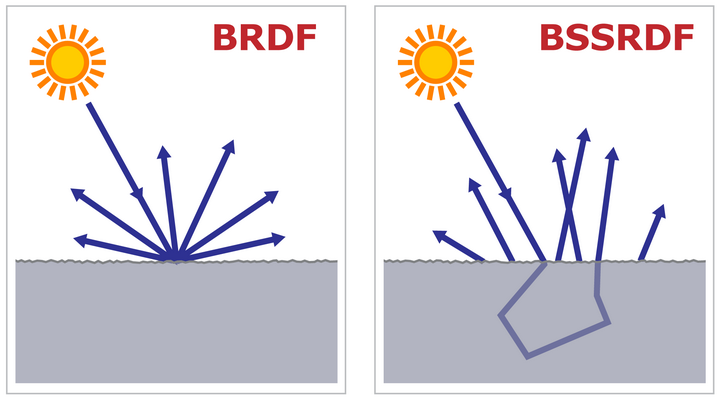
\includegraphics[scale=0.5]{./Pictures/BSSRDF_BRDF.png}
    \caption{BRDF vs BSSRDF Comparison}
    \label{bssrdf_brdf}
  \end{center}
\end{figure}

The BSSRDF, $S$, relates the outgoing radiance, $L _o(x _o, \vec{\omega} _o)$ at the point $x _o$ in the direction $\vec{x} _o$, to the incident flux, $\Phi _i(x _i, \vec{\omega} _i)$, at the point $x _i$ from direction $\vec{\omega} _i$:

\begin{equation}
dL _o(x _o, \vec{\omega} _o) = S(x _i, \vec{\omega} _i; x _o, \vec{\omega} _o) d\Phi _i(x _i, \vec{\omega} _i)
\end{equation}

Given a BSSRDF, the outgoing radiance is computed by integrating the incident radiance over incoming directions and area, $A$:

\begin{equation}
L _o(x _o, \vec{\omega} _o) = 
\int_{A}\int _{2\pi} S(x _i, \vec{\omega} _i; x _o, \vec{\omega} _o) L_i(x_i, \vec{\omega_i})(\vec{n} \cdotp \vec{\omega}_i) \,d\omega_i \,dA(x_i)
\end{equation}

\section{Model}
Introduce the model; mention that it comes from the previous paper and more information can be found in there;

\subsection{The Diffusion Approximation}
The idea: comes from medical sciences - the dipole; the importance of multiple scattering - dominant
\subsection{Two-Pass Technique for Evaluating the Diffusion Approximation}
Introduction to the two pass techinque: key idea, to make it faster decouple the computation of irradiance...
\subsubsection{Sampling the Irradiance}
Good to have uniform distribution of sample points - the authors used Turk's algorithm; Number of points defined by lu and total area; usage of GI techniques;
equations
\subsubsection{Evaluating the Diffusion Approximation}
Can be used directly - heavy, lots of points; speak about the 3 options; hierarchical evaluation: best of both worlds; storage on the tree; subdivision criterion; computation of the radiant exitance and finally computing the Lo for each point.
input parameters: sigmas

\section{Implementation}
The implementation was initially divided into two parts: uniformly sampling the points and the hierarchical evaluation. However, the point sampling took much more time than it was expected and the work continued in that very same direction. It should be noticed that both of us knew the other one's part and the for several times we worked together in only one part.\linebreak
The code versioning and backup was done using Google Project Hosting SVN server\textbf{  XXX SHOULD WE PUT HERE THE LINK ???? XXX}. In this way the synchronization of the code made by both was easy, secure and straightforward.

\subsection{Renderer}
The initial proposal for a renderer mentioned a Pixar's RenderMan$^{\textregistered}$ compliant opensource renderer. The choice made was Pixie XXX Ref to it XXX. The framework seemed to be pretty stable and up-to-date. After several days studying RenderMan$^{\textregistered}$'s specification and trying to understand Pixie's implementation we decided that it was unrealistic to use it due to the lack of documentation and due to Renderman's low support for ray-tracing.\linebreak
The final choice for a renderer was then PBRT. The documentation was excellent and the renderer seemed to be widely used on the academic environment.\linebreak
\textbf{ XXX SHOULD WE TALK HERE ABOUT PBRT'S SET UP TIME ??? XXX }
Although PBRT is thought to be extended given its plugin nature, modelling a BSSRDF isn't that straightforward (as also mentioned myb the authors on the reference book). Several changes to its core must be made in order to get access to different information. The major changes are related with the {\it Shape, Material, GeometricPrimitive, Triangle and TriangleMesh} objects.

\subsection{First Pass - Sampling The Irradiance}
Turk's algorithm explanation; usage of basic MC estimator; storage of points on the octree - next section.

\subsection{Second Pass - Evaluating the Diffusion Approximation}

For the hierarchical evaluation, like the authors of the paper, we used an octree to store all our irradiance samples. In order to evaluate the total radiosity at a location $x$ on the surface of the object, the octree must be traversed starting from the root. For each voxel we test if:


\begin{figure}[tbh]
\centering
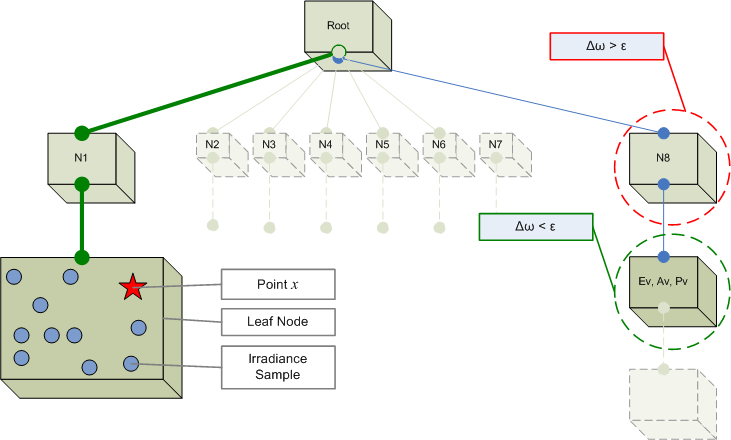
\includegraphics[scale=0.5]{./Pictures/Octree.png}
\caption{}
\label{Hierarchical Evaluation}
\end{figure}

octree - add and lookup; one or two schemes; the epsilon factor;

\section{Results}
\section{Conclusion}

% ### BIBLIOGRAPHY ###
\begin{thebibliography}{99}

%
% WIKI REFERENCE
%

\bibitem{WelshParallax} Welsh, Terry, 2004, {\it Parallax Mapping with Offset Limiting: A PerPixel Approximation of Uneven Surfaces}

\bibitem{TatarchukParallax} Tatarchuk, Natalya, 2006, Dynamic Parallax Occlusion Mapping with Approximate Soft Shadows. In {\it Proceedings of the 2006 symposium on Interactive 3D graphics and games SI3D '06}, ACM Press pp. 63-69.

\end{thebibliography}


\end{document}
